\documentclass[12pt]{article}
\usepackage{CJKutf8}
\usepackage{graphicx}
\begin{document}

\begin{CJK}{UTF8}{gbsn}
\section{1}
误码率太高
\begin{itemize}
  \item 附近有同频信号干扰,远离干扰源或者修改频率、信道避开干扰;
  \item 电源不理想也可能造成乱码,务必保证电源的可靠性;
  \item 延长线、馈线品质差或太长,也会造成误码率偏高。
\end{itemize}
\section{2}
ZigBee网络中通信,单包数据发送周期不能过快 (一般建议在 1 秒以上) ,过快可能造成数据的丢失。
特别注意,网络中节点太多,广播周期过快可能会造成网络不稳定。 

\section{0-router-metting room}
  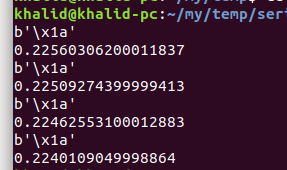
\includegraphics[width=\textwidth]{./0-router-metting-room.png}
\section{2-router-metting room}
  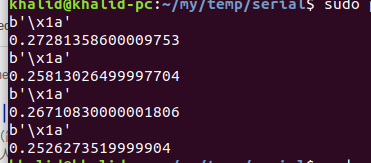
\includegraphics[width=\textwidth]{./2-router-metting-room.png}

\section{3-router-metting room}
  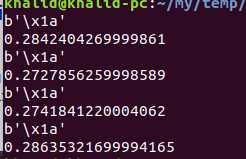
\includegraphics[width=\textwidth]{./3-router-metting-room.png}
% 1.
% b'\x1a'
% 0.5892778759998691
% b'\x1a'
% 0.5939465219998965
% b'\x1a'
% 0.29362439600026846
% b'\x1a'
% 0.29169378500000676
% 
% 2.
% b'\x1a'
% 0.29123983599993153
% b'\x1a'
% 0.2876203769997119
% b'\x1a'
% 0.28699319999986983
% b'\x1a'
% 0.2868535679999695
\section{overview of experiment}
  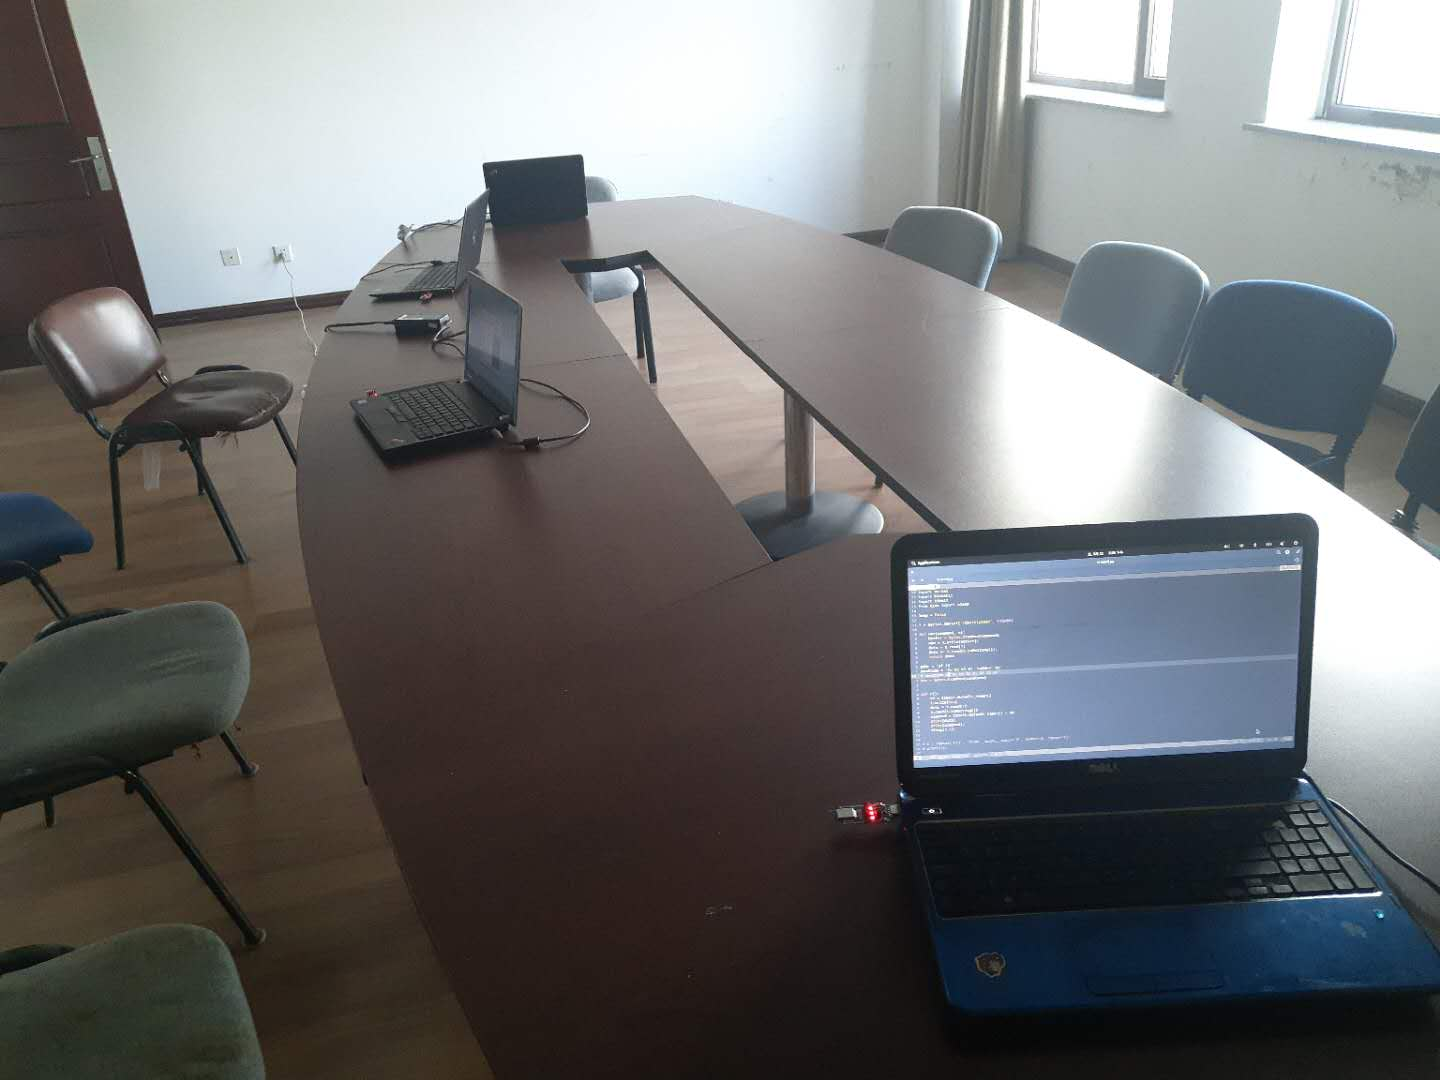
\includegraphics[width=\textwidth]{./overview-from-server.jpg}
  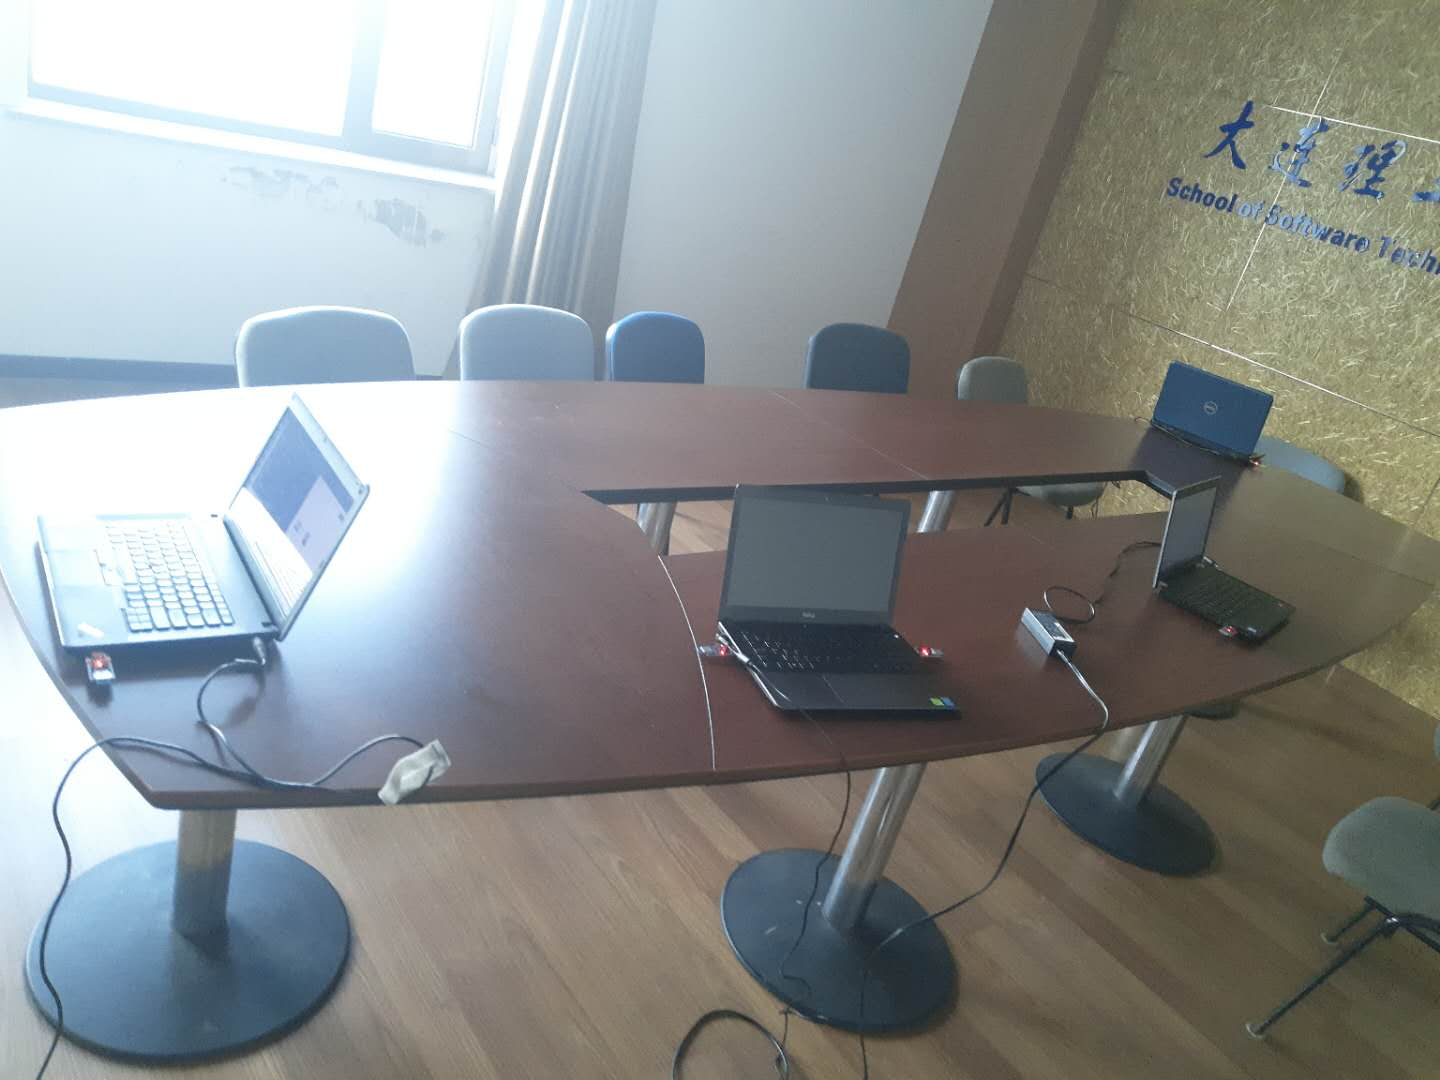
\includegraphics[width=\textwidth]{./overview-from-side.jpg}
  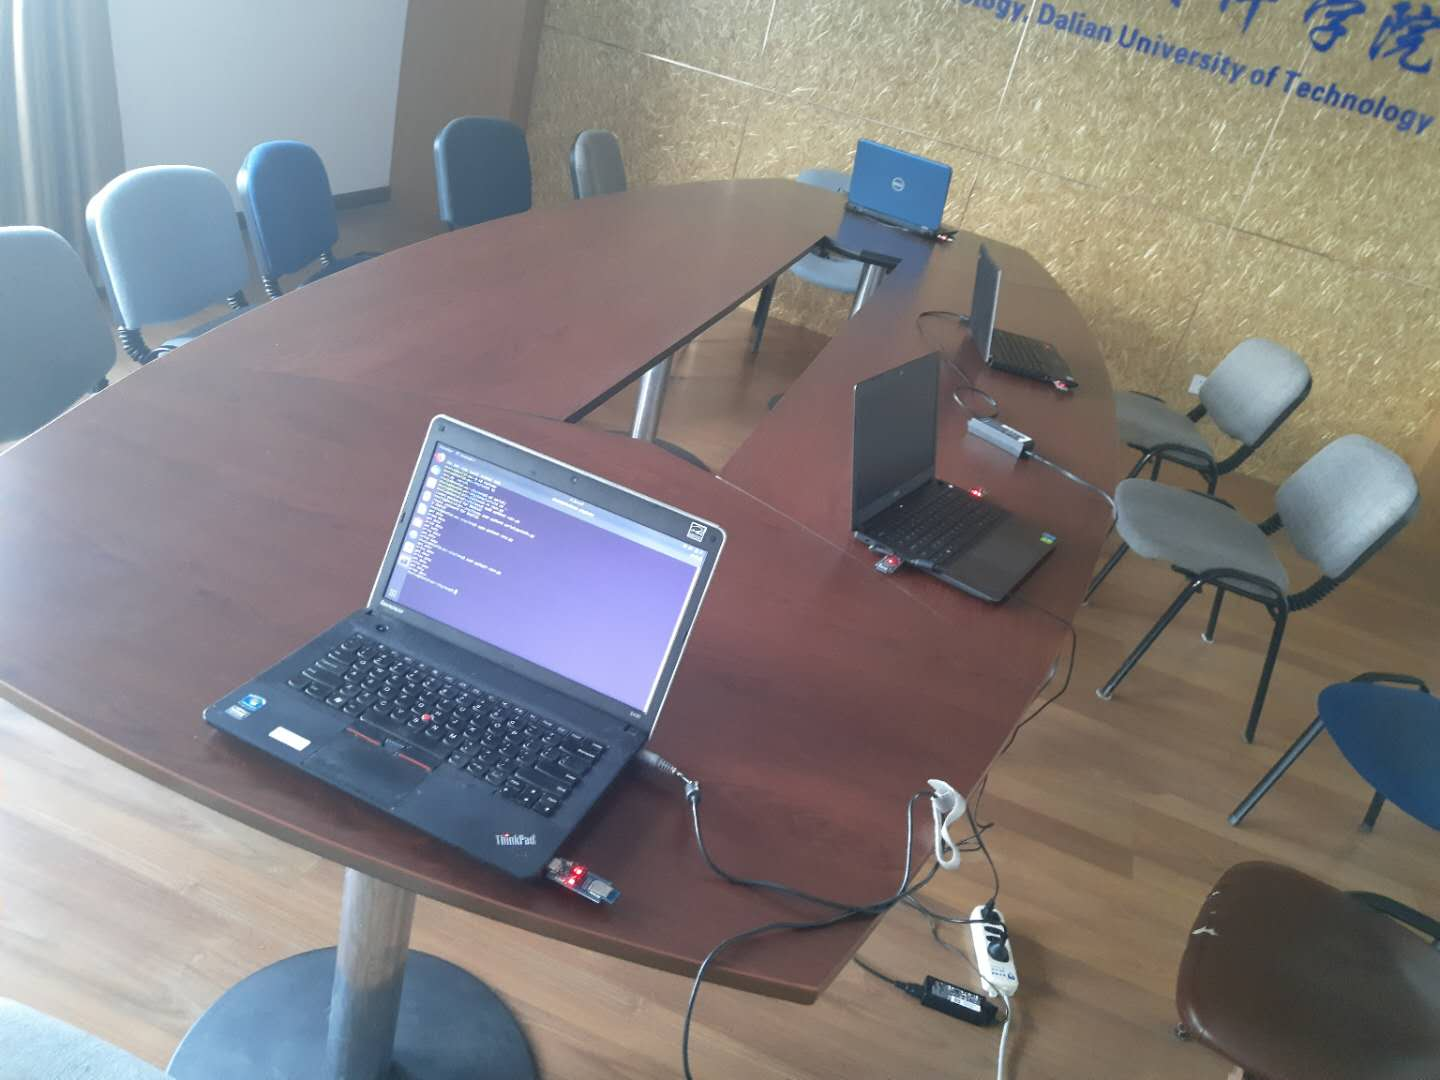
\includegraphics[width=\textwidth]{./overview-from-endnode.jpg}
\section{node}
  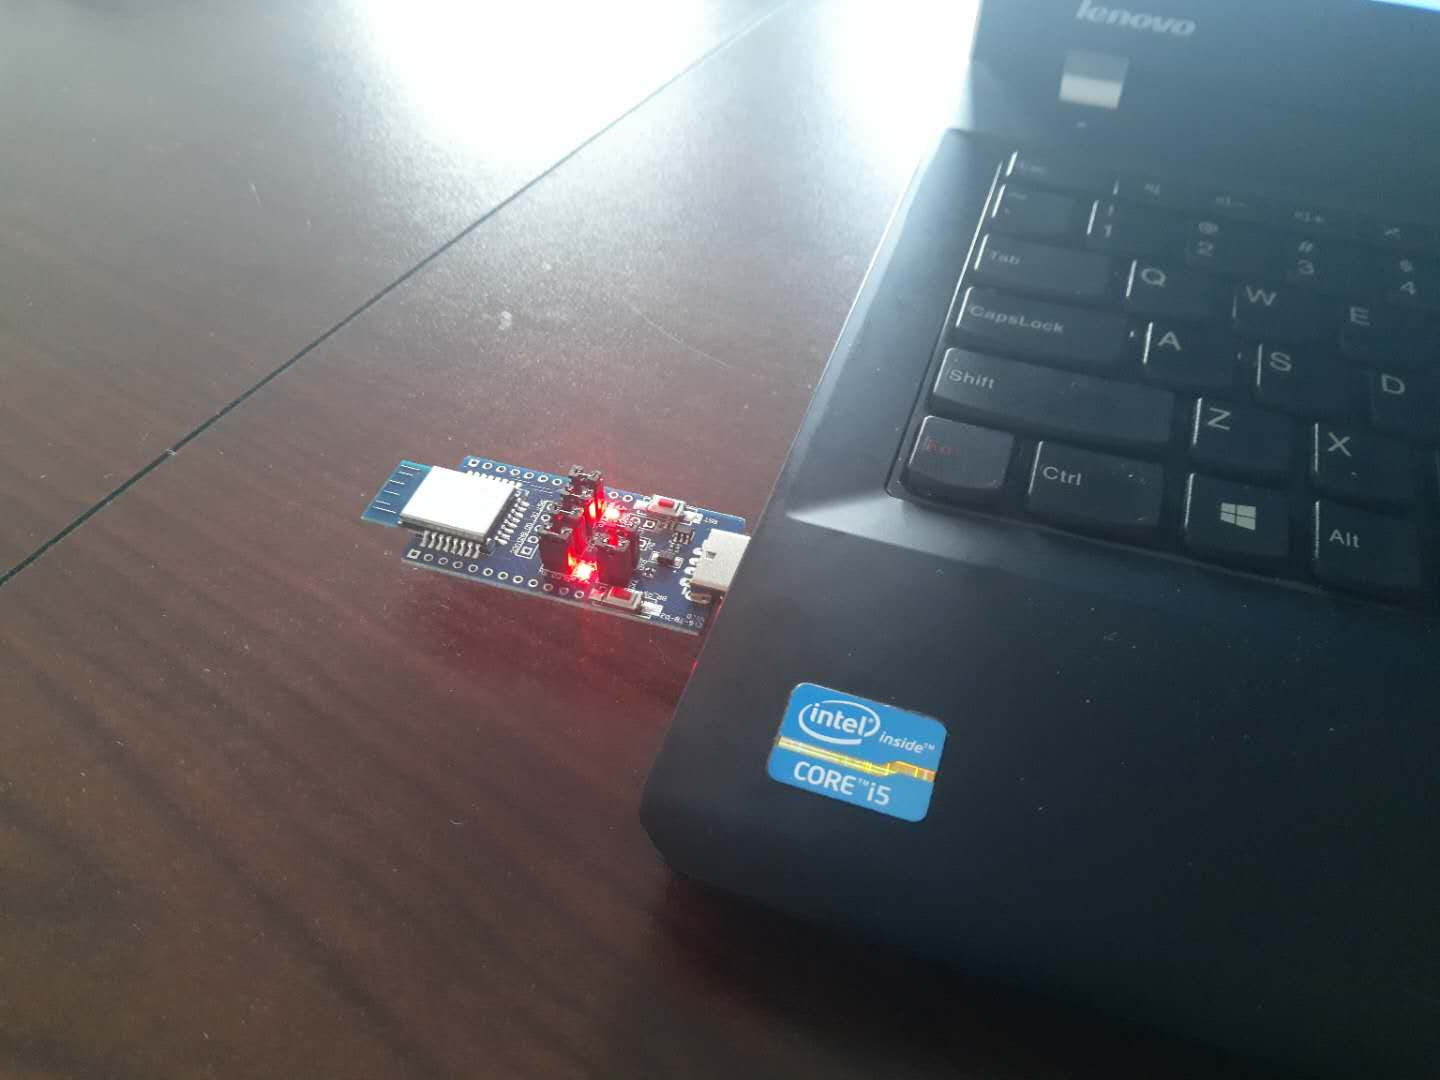
\includegraphics[width=\textwidth]{./aNode.jpg}
  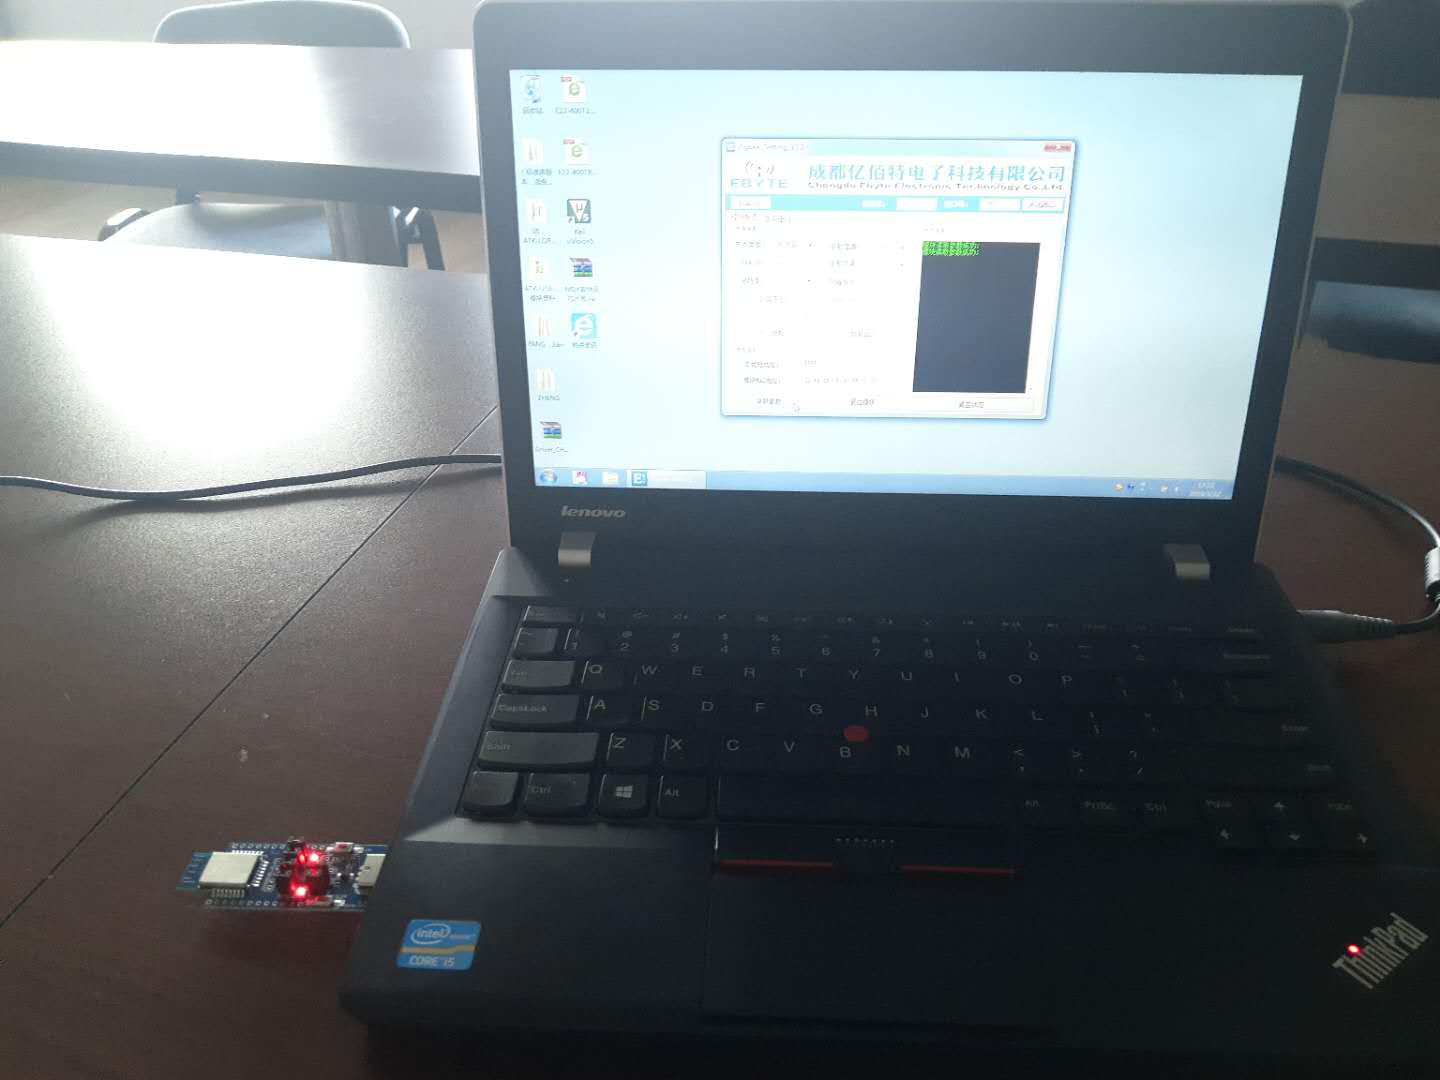
\includegraphics[width=\textwidth]{./aNodeWithlaptop.jpg}

\end{CJK}
\end{document}
